\chapter{Estudio sobre el acero libre de intersticiales}\label{C:IF}
\graphicspath{{./figs/03_IF/}}
\chapterquote{The void is without substance but cuts like steel.}{Mark Rosewater}

En este capítulo se estudia la microestructura de un acero libre de intersticiales (IF) que fue laminado hasta lograr una reducción de la sección transversal del 70\,\%.
Este acero fue obtenido comercialmente, y posee la textura propia de un material BCC laminado, con dos componentes predominantes: la fibra $\alpha$ y la fibra $\gamma$.

Se eligió este acero por su importancia en la industria automotriz y porque existe cierto consenso acerca de cómo se desarrolla la microestructura de este material en condiciones de laminado, donde se espera que los defectos se acumulan predominantemente en la fibra $\gamma$.

El material fue estudiado por dos técnicas independientes, EBSD y XRD, y los datos de XRD fueron analizados dos modelos diferentes, el CMWP y empleando figuras de polos generalizadas a partir de los anchos de los picos de difracción, y se encontró que este modelo es que el que mejor representa lo que ocurre con la microestructura del material, ya que no sólo responde a lo que se esperaba según la experiencia previa, sino que además va de acuerdo con lo que se pudo concluir a partir de los experimentos de EBSD.

\section{Textura}\label{S:IFText}
Mediciones de textura fueron realizadas según lo descrito en la Sec. \ref{S:MatXRD} y las figuras de polos experimentales que se muestran en la Fig. \ref{fig:IFTextRawRec}-a fueron analizadas por una rutina de inversión FP-FDO del software MTEX.
Una vez obtenida la FDO, que se puede ver en la Fig. \ref{fig:IFODF}, se empleó la misma para calcular independientemente las mismas FP medidas y se compararon los datos experimentales con los recalculados que se muestran en la Fig \ref{fig:IFTextRawRec}-b.

\begin{figure}[!htb]
  \centering
  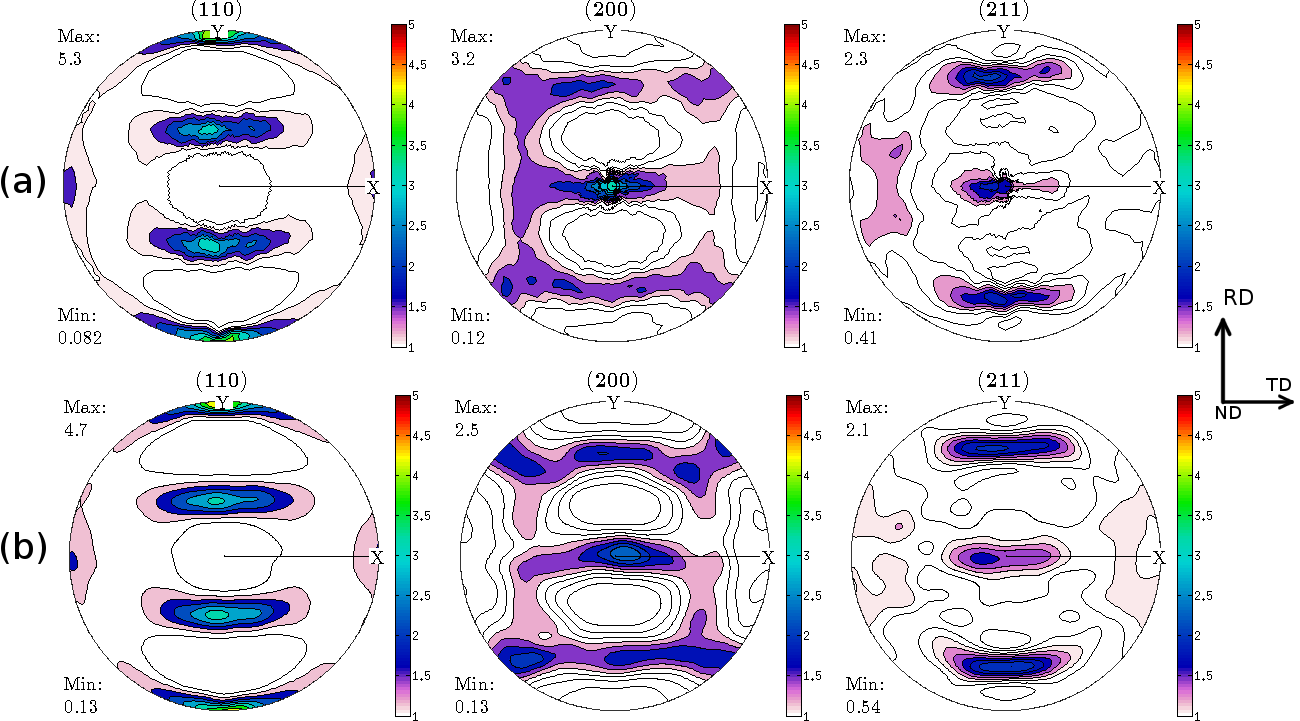
\includegraphics[width=0.9\textwidth]{IF75_Text_RawRec}
  \caption{(a) Figuras de polos medidas para el acero libre de intersticiales. (b) Figuras de polos recalculadas luego de calcular la FDO a partir de las figuras de polos medidas. Puede apreciarse un buen acuerdo entre las figuras de polos medidas y las recalculadas, tanto en las características cualitativas como cuantitativas de las figuras, lo que constituye una prueba indirecta de la buena calidad de los datos. En cuanto a la textura observada, se aprecian claramente los polos producidos  por las fibras $\alpha$ y $\gamma$ que suelen generarse en este tipo de aceros luego de los procesos de laminado.}
  \label{fig:IFTextRawRec}
\end{figure}

Puede apreciarse que la FP recalculada tiene prácticamente la misma forma que la experimental, lo que habla de la consistencia que guardan entre sí las diferentes FPs.
Adicionalmente puede verse que las intensidades de las FPs recalculadas son similares a la de las experimentales, aunque las intensidades máximas son siempre un poco menores en las FP recalculadas, lo que constituye una discrepancia esperable teniendo en cuenta que las FDO son reconstruidas a partir de calcular los coeficientes de un desarrollo en serie, lo que suele ``achatar'' los máximos de la FDO, lo que resulta a su vez en una reducción de los máximos observados en la FP.

En la FP (110) puede verse una de las componentes característica de este muchos aceros, la denominada \textit{fibra} $\alpha$ que consta de todos los cristales que tienen su dirección [110] en la dirección de laminado sin importar su giro alrededor de ese eje. Esto se manifiesta como un máximo en la intesidad en la FP (110) en la dirección RD.

Por otro lado en la misma FP se pueden ver dos máximos locales simétricos que forman un ángulo de unos 45\,$^{\circ}$ con el plano ND-TD, y que tienen forma de lóbulos alargados en la dirección TD. 
Estos máximos corresponden a otra componente importante en los aceros que se denomina \textit{fibra} $\gamma$ y se construye de una manera similar a la $\alpha$, sólo que en este caso se trata de los cristales con su dirección [111] paralela a ND.

\begin{figure}[!htb]
  \centering
  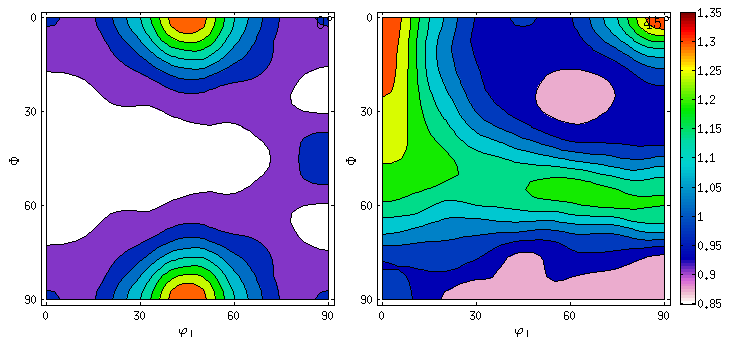
\includegraphics[width=0.9\textwidth]{IF75R_odf_orto}
  \caption{FDO calculada para el acero IF. Se muestran las secciones $\phi_2 \ = \ 0$\,$^{\circ}$ y $\phi_2 \ = \ 45$\,$^{\circ}$. En la sección $\phi_2 \ = \ 45$\,$^{\circ}$ pueden apreciarse claramente las fibras $\alpha$ y $\gamma$.}
  \label{fig:IFODF}
\end{figure}

En la Fig. \ref{fig:IFODF} se representa la FDO del acero IF, calculada a partir de los datos de la Fig. \ref{fig:IFTextRawRec}.
Como se explicó en la Sec. \ref{S:Text}, las orientaciones se represetan mediante los Ángulos de Euler, y como la FDO depende de tres ángulos, se conviene generalmente en representar la misma en secciones que cumplen $\phi_2 \ = \ cte.$, mientras que las coordenadas $\phi_1$ y $\Phi$ se representan en el eje de las abscisas y de las ordenadas, respectivamente.
En este caso se muestran las dos secciones más importantes para este tipo de materiales, las secciones $\phi_2 \ = \ 0$\,$^{\circ}$ y $\phi_2 \ = \ 45$\,$^{\circ}$.
Adicionalmente, se restringe representar la coordenada $\phi_1$ en el rango 0\,$^{\circ}$ a 90\,$^{\circ}$ teniendo en cuenta que la red BCC tiene una simetría cúbica y que los procesos de laminado tienen una simetría de tipo ortotrópica, haciendo redundante la información que se encuentra fuera del intervalo mostrado.

En la sección $\phi_2 \ = \ 45$\,$^{\circ}$ pueden apreciarse las fibras $\alpha$ y $\gamma$ con claridad. 
La primera consiste de las orientaciones que van desde $\Phi \ = \ 0$\,$^{\circ}$ hasta aproximadamente 57\,$^{\circ}$, manteniendo $\phi_1 \ = \ 0$\,$^{\circ}$.
La segunda, en cambio, mantiene el ángulo $\Phi \ = \ 57$\,$^{\circ}$ y barre $\phi_1$ en todo su rango. El valor de 57\,$^{\circ}$ no es casual, sino que proviene del ángulo que forma la dirección [111] con la [100].
Los máximos que se observan en la seccion $\phi_2 \ = \ 0$\,$^{\circ}$ corresponden a las orientaciones de la fibra $\alpha$.

A partir de analizar la Fig. \ref{fig:IFODF} puede apreciarse que la gran mayoría de los cristales de este material se encuentran distribuidos entre las fibras $\alpha$ y $\gamma$, habiendo una proporción un poco mayor al comienzo de la fibra $\alpha$, tal como es de esperarse en este tipo de materiales cuando son sometidos a deformaciones como el laminado.

En este contexto, queda claro que no todas las orientaciones están igualmente representadas en este material, por lo que se espera que la microestructura también exhiba algún tipo de anisotropía.
En las dos secciones que siguen se analizará la anisotropía de la microestructura a partir de dos modelos, el de Langford y el CMWP, y se observará que ambos dan lugar a interpretaciones diferentes, que se tratarán de compatibilizar con los resultados de las mediciones de EBSD (Sec \ref{S:IFEBSD}).

\section{Estudio de la microestructura por el método CMWP}\label{S:IFCMWP}
El análisis siguiendo el método CMWP tiene dos diferencias fundamentales con el método de Langford, ya que al tratarse de un método bottom-up los resultados que se obtienen son inherentemente cuantitativos, además, como el método supone que el ensanchamiento anisotrópico se debe solamente al cambio de los factores de contraste de las dislocaciones, produce resultados que permiten caracterizar la microestructura sólo como función de la orientación de la muestra, promediando la información que se obtiene de cada uno de los picos de un difractograma. 
Este enfoque parece intuitivamente acertado cuando se quiere estudiar la forma de los granos, ya que se sabe que los mismos tienden a adquirir una morfología dada por el proceso de deformación, más que por su orientación cristalográfica.
Qué tan acertado es este modelo cuando se estudia la acumulación de dislocaciones es un tema abierto hoy en día.

En las Figs. \ref{fig:IFCMWPSize}-a y \ref{fig:IFCMWPSize}-b puede observarse cómo varía la distribución de tamaño de las cristalitas con la orientación de la muestra a través de los parámetros fundamentales de la distribución: su moda y su dispersión.
A partir de estos parámetros se puede calcular trivialmente el tamaño promedio de cristalita de la muestra para cada orientación, que se exhibe en la Fig. \ref{fig:IFCMWPSize}-c.

\begin{figure}[!htb]
  \centering
  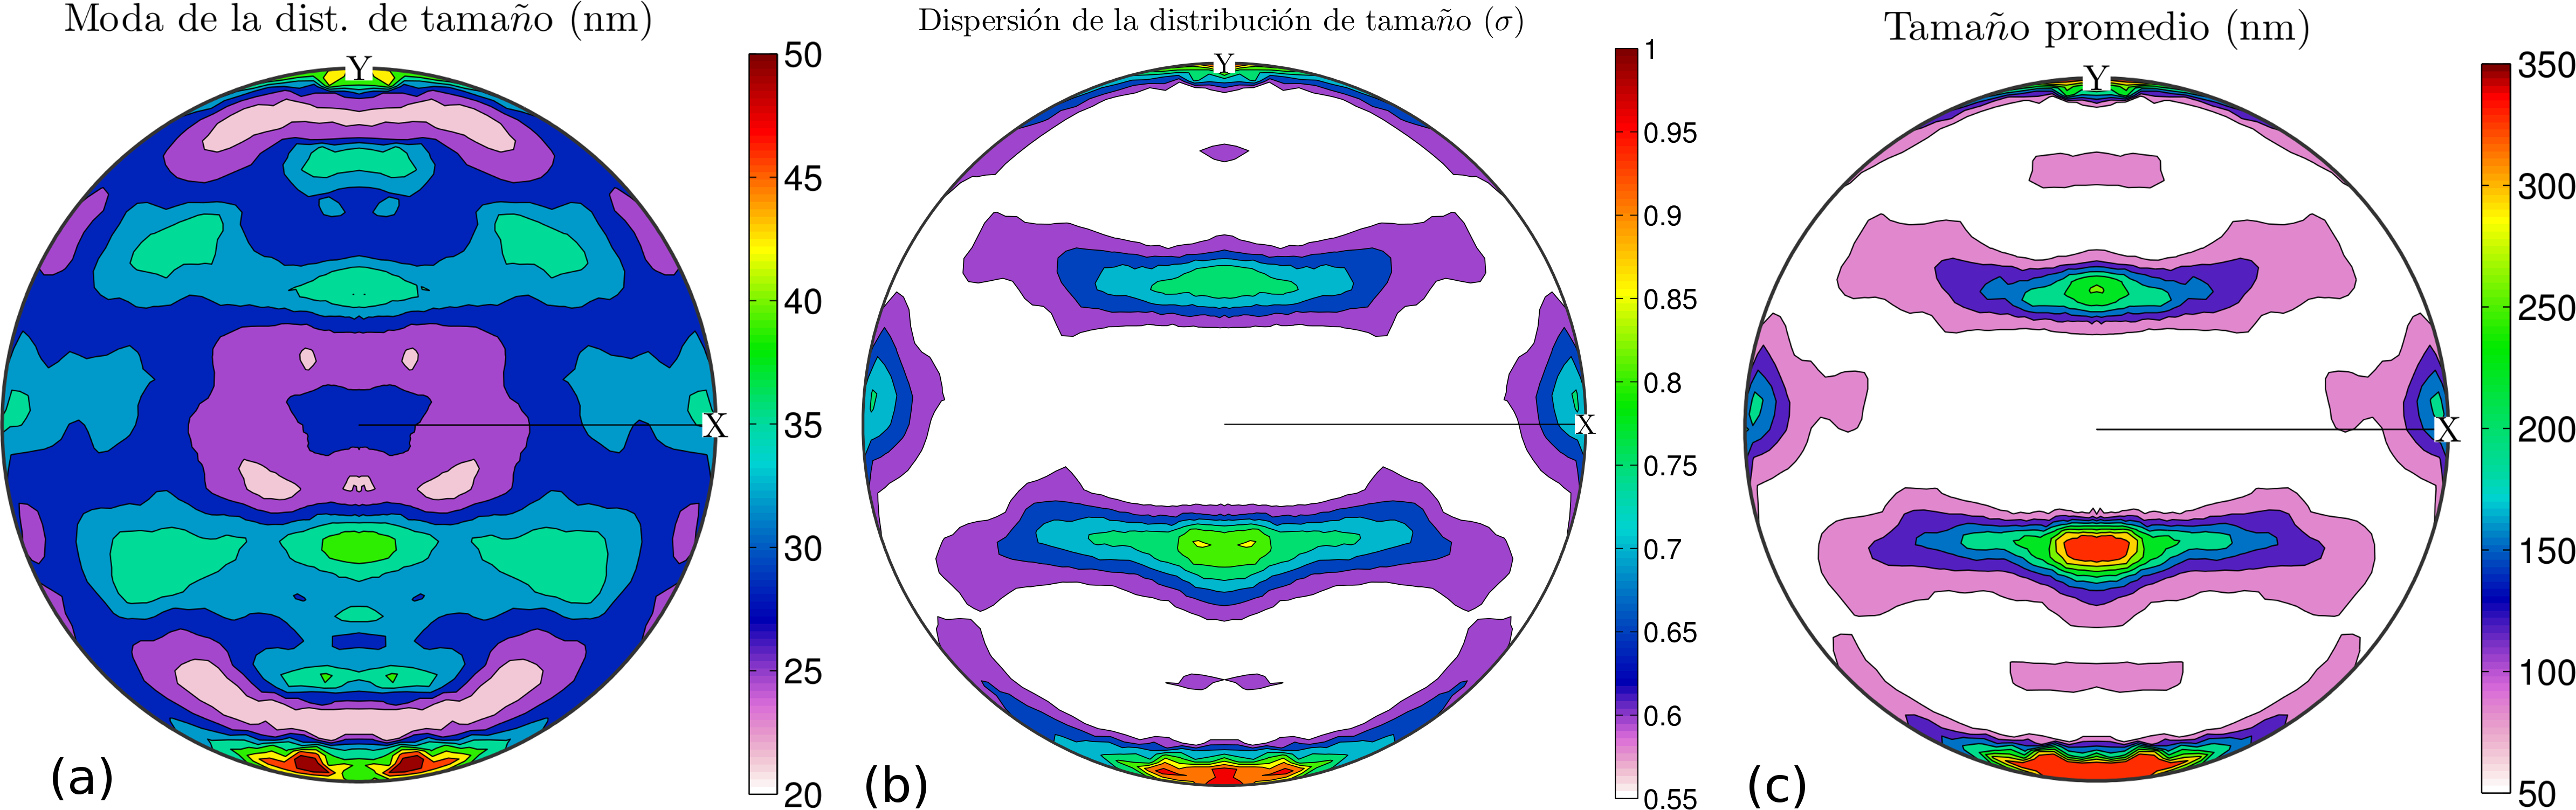
\includegraphics[width=\textwidth]{CMWP_size}
  \caption{Figuras de polos de la moda de la distribución lognormal de tamaño de cristalita (a), dispersión de dicha distribución (b) y tamaño medio de cristalita(c).}
  \label{fig:IFCMWPSize}
\end{figure}

Al observar la FPG de tamaño de dominio puede observarse cierto parecido con la FP (110) de la Fig. \ref{fig:IFTextRawRec}, lo que podría interpretarse que son los planos $\{110\}$ los que comandan el tamaño de las cristalitas, y que las mismas tienen una variación importante en su tamaño promedio, estando el mismo en el rango de los 50\,nm a los 350\,nm, estando los máximos en los mismos lugares que los máximos de la FP (110) del acero IF.

Para estudiar la acumulación de dislocaciones en el acero IF el método CMWP provee más información que en el caso de la distribución de tamaño, ya que no sólo se puede obtener la densidad de dislocaciones como función de la orientación de la muestra (Fig. \ref{fig:IFCMWPrho}-b), sino que también se puede calcular cómo varía el carácter de dichas dislocaciones a través del factor $q$ de la Ec. \ref{eq:Cav2} (Fig. \ref{fig:IFCMWPrho}-a).
Una vez determinado el carácter y cantidad de dislocaciones, se puede determinar hasta donde se extiende el campo de deformación producido por las mismas (Fig. \ref{fig:IFCMWPRe}-a) y si éstas se encuentran dispersas aleatoria y uniformemente en la cristalita o si interactúan entre ellas formando arreglos compactos.
Esta última característica es determinada por el facto de Wilkens que fue definido al final de la Sec. \ref{SS:XRD-LPA}, y que se encuentra graficado en la Fig. \ref{fig:IFCMWPRe}-b.

\begin{figure}[!htb]
  \centering
  \includegraphics[width=0.7\textwidth]{CMWP_rho}
  \caption{(a) Figura de polo generalizadas del factor $q$ (según Ec. \ref{eq:Cav2}). (b) Figura de polos de densidad de dislocaciones.}
  \label{fig:IFCMWPrho}
\end{figure}

Si se compara la forma de la FP de densidad de dislocaciones con la de tamaño de cristalita puede notarse que ambas son cualitativamente similares, lo que implicaría que los dominios más grandes son los que han acumulado más dislocaciones.
La forma de la FP de $q$ es bien diferente a las FP anteriores, teniendo un valor de aproximadamente 1 en todo el rango, incrementándose a 2.5 en las direcciones RD y TD, lo que indicaría que las dislocaciones tienden a tener un carácter de hélice en esas direcciones de la muestra.

\begin{figure}[!htb]
  \centering
  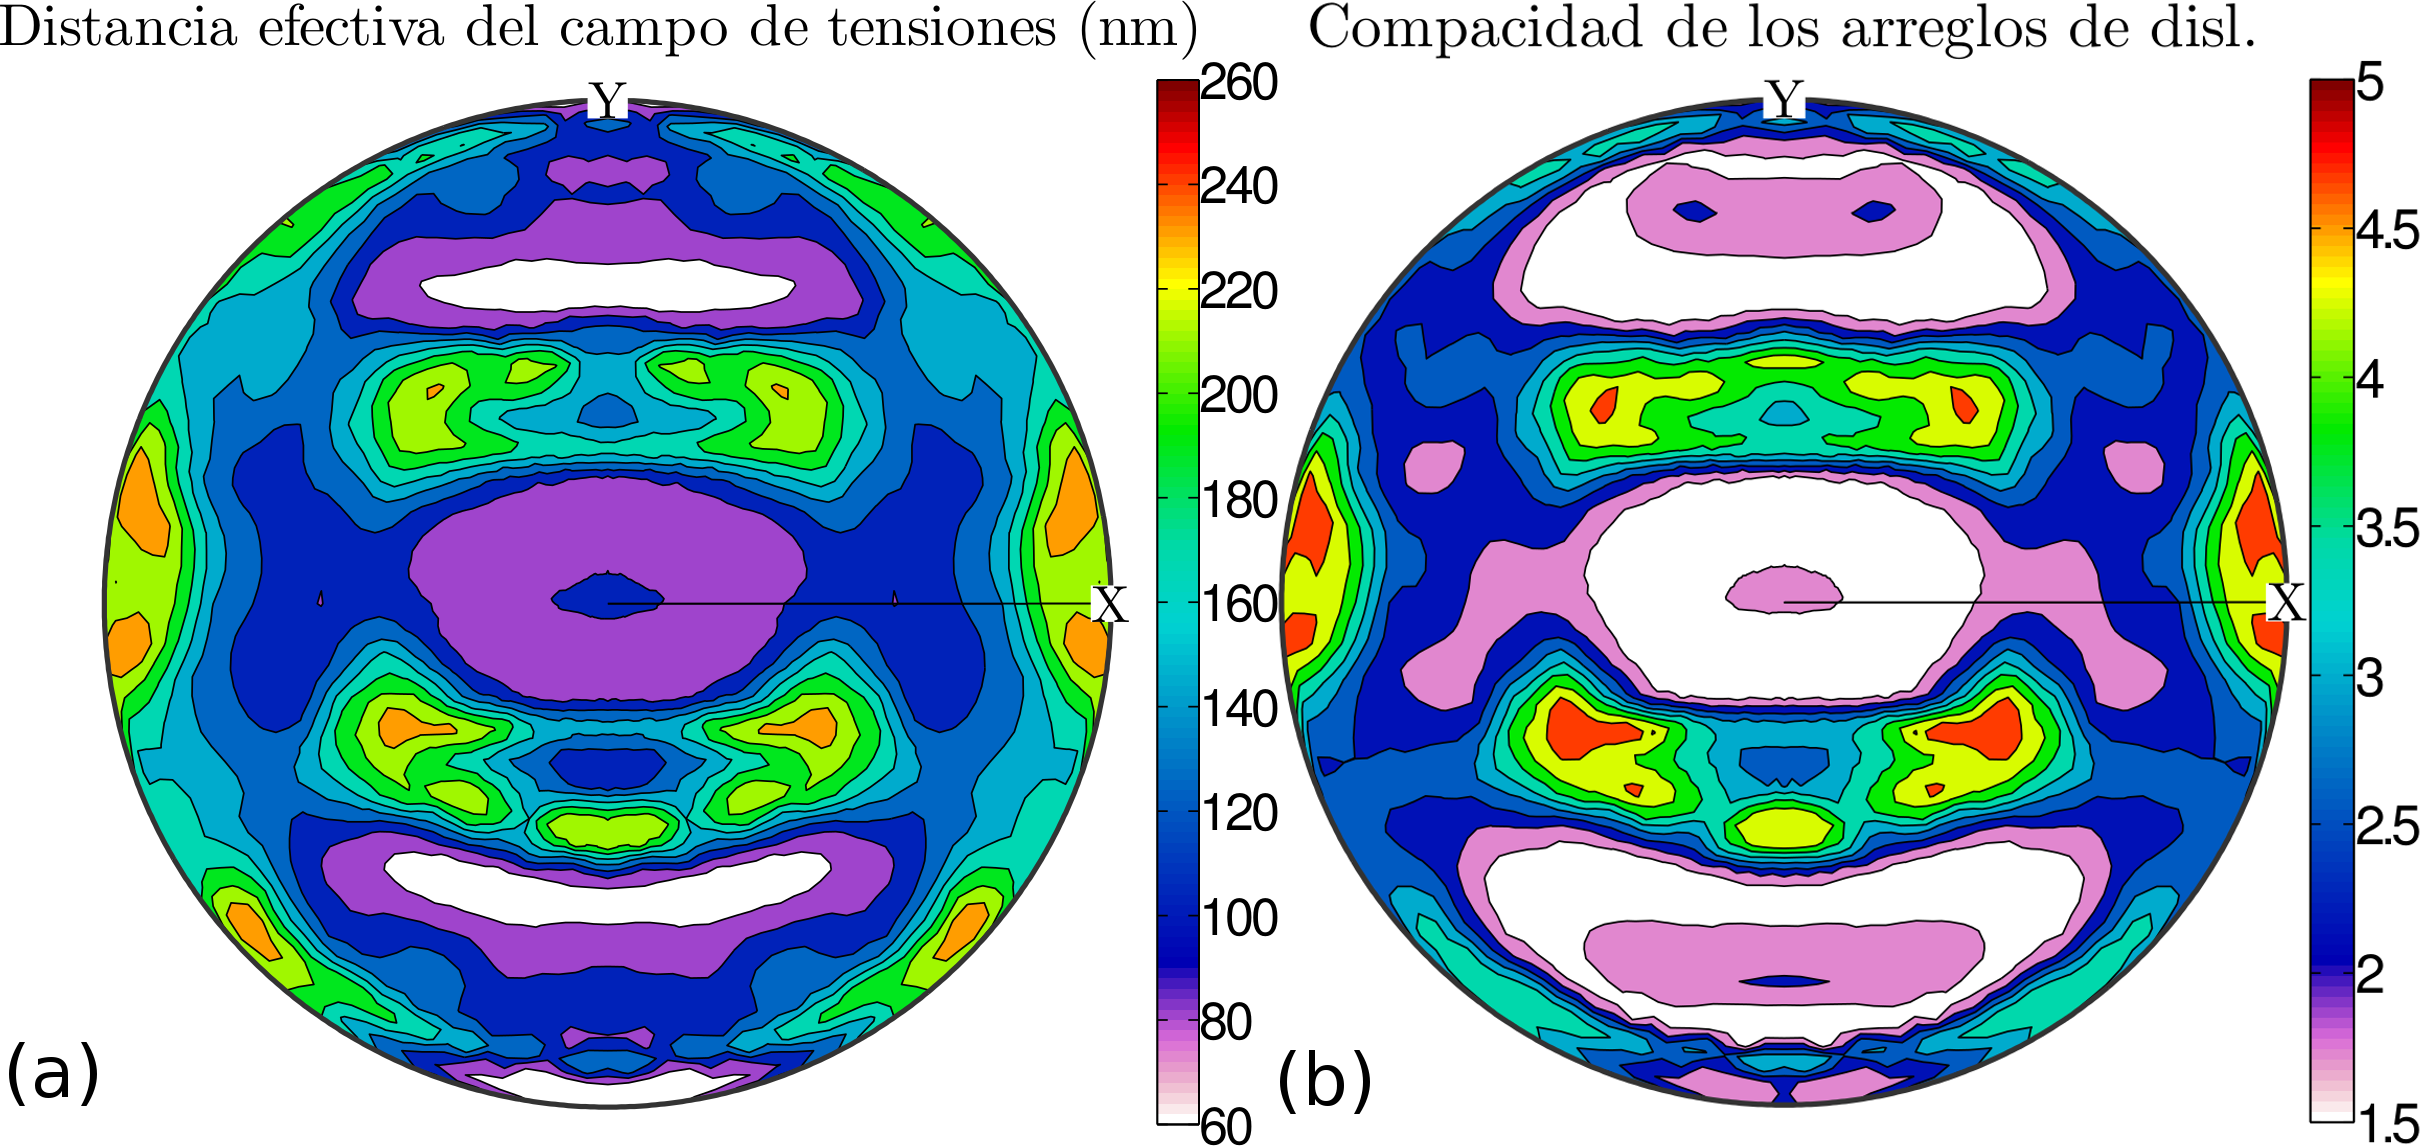
\includegraphics[width=0.7\textwidth]{CMWP_Re}
  \caption{Figuras de polos de (a) distancia del campo de distorsión producido por las dislocaciones y (b) Factor de Wilkens, indicador de la compacidad de los arreglos de dislocaciones.}
  \label{fig:IFCMWPRe}
\end{figure}

Por otro lado, tanto la FP de longitud del campo de dislocaciones como la de compacidad de los arreglos son muy similares entre sí, a la vez que a las FP de $\rho$ y tamaño, lo que significa que las orientaciones de muestra paralelas a la familia de planos (110) tienen dominios más grandes, con el máximo de densidad de dislocaciones, y que las mismas interactúan débilmente entre sí, generando un campo de distorsión con un alcance de uno 200 nm en promedio. Nótese que el alcance del campo de tensiones de las dislocaciones es similar a la del tamaño de dominio, lo que constituiría el máximo valor esperable para dicha distancia.

\section{Estudio de la microestructura por el método de Langford y figuras de polos generalizadas}\label{S:IFLANG}
Como se explicó en la Sec. \ref{SS:MatPost}, de los experimentos de difracción no sólo se extrajo la intensidad de los picos que se empleó para medir la textura de los materiales, sino que también se extrajo información sobre la forma del pico, en particular el FWHM.
Los FWHM obtenidos para cada pico en la orientación de la muestra fueron graficados en figuras de polos generalizadas, como las que se muestran en la Fig. \ref{fig:IFFWHMRawRec}.
La contribución instrumental al FWHM fue tratada según lo explicado en la Sec. \ref{SS:inst} y se emplearon dichas FPG para construir una FDOG, tal como se explicó en la Sec. \ref{SS:ODFG}.

\begin{figure}[!htb]
  \centering
  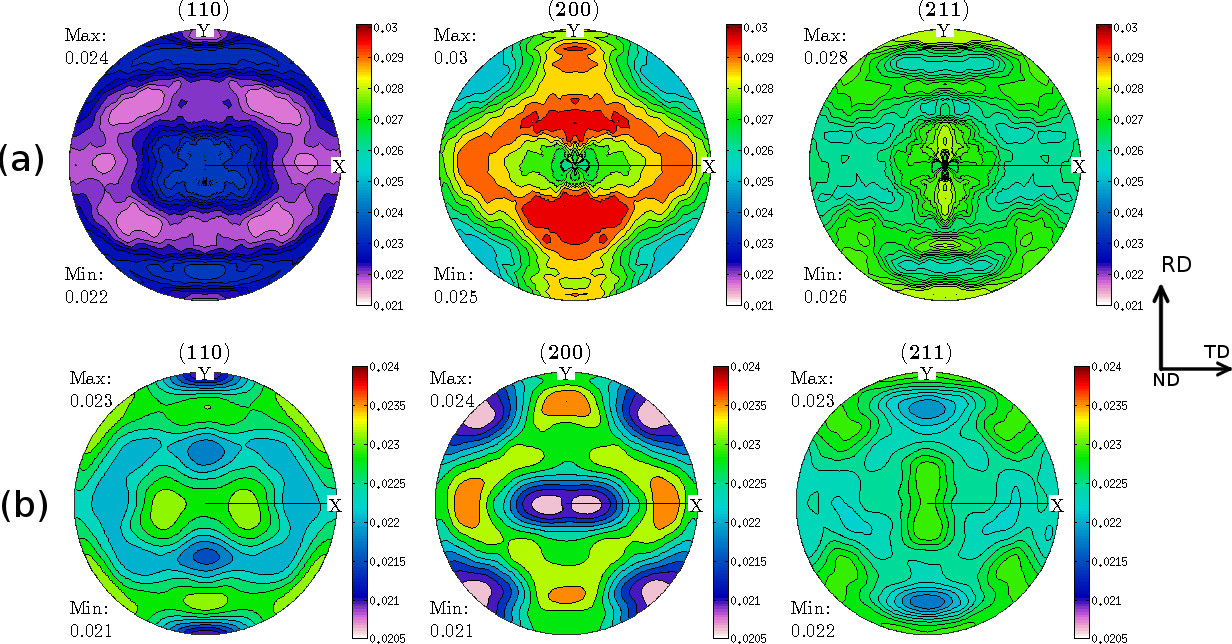
\includegraphics[width=\textwidth]{IF75_FWHM_RawRec}
  \caption{(a) Figuras de polos generalizadas medidas para el acero libre de intersticiales. (b) Figuras de polos generalizadas recalculadas luego de calcular la FDOG a partir de las figuras de polos medidas. Puede apreciarse un acuerdo cualitativo entre las figuras de polos medidas y las recalculadas, lo que constituye una prueba indirecta de lo consistente de la suposición de que el ancho de pico es una buena cantidad para representar la anisotropía de microestructura. Puede observarse cierta complementariedad entre estas figuras y las figuras de polos de la Fig. \ref{fig:IFTextRawRec}, lo que indicaría que las orientaciones favorecidas por la textura habrían acumulado menos defectos.}
  \label{fig:IFFWHMRawRec}
\end{figure}

Para determinar si los FWHM medidos responden de alguna manera a la textura cristalográfica se compararon las FPs con las FPGs, para ver si entre las mismas hay algún tipo de correlación.
Al comparar la Fig. \ref{fig:IFTextRawRec}-a con la Fig. \ref{fig:IFFWHMRawRec}-a puede apreciarse cierta complementariedad entre ambas, lo que se podría interpretar como que las orientaciones favorecidas por la textura son aquellas que acumularon menos defectos.
Sin embargo, como en las FP y las FPG se observan mezclas de diferentes orientaciones, no se puede afirmar si la fibra $\alpha$ y la $\gamma$ acumulan igual cantidad de defectos o no.

La otra manera que se empleó para ver qué tan bien los FWHM sonn representables por una FDOG fue pasar los datos de la Fig. \ref{fig:IFFWHMRawRec}-a por la misma rutina de reconstrucción de ODF que se aplicó a las texturas y luego, a partir de dicha FDOG recalcular las FPGs, y comparar ese resultado con los datos experimentales.

Al comparar los datos experimentales que aparecen en la Fig. \ref{fig:IFFWHMRawRec}-a con los recalculados de la Fig. \ref{fig:IFFWHMRawRec}-b puede apreciarse que existe un acuerdo cualitativo muy bueno entre ambas figuras, aunque las intensidades máximas y mínimas se modifican al pasar de los datos experimentales a los recalculados.
Teniendo en cuenta lo observado, se decidió emplear la FDOG obtenida para tratar de dilucidar diferencias cualitativas que pudieran aparecer en la microestructura de diferentes componentes de textura, dejando de lado la interpretación cuantitativa de los resultados.

El siguiente paso del estudio fue comparar la FDO con la FDOG de FWHM que se puede observar en la Fig. \ref{fig:IFODFComp}-b.
La Fig. \ref{fig:IFODFComp}-a es la misma FDO que se ve en la Fig. \ref{fig:IFODF}, que se decidió mostrar junto a la FDOG para facilitar al lector la comparación de las mismas.
\begin{figure}[!htb]
  \centering
  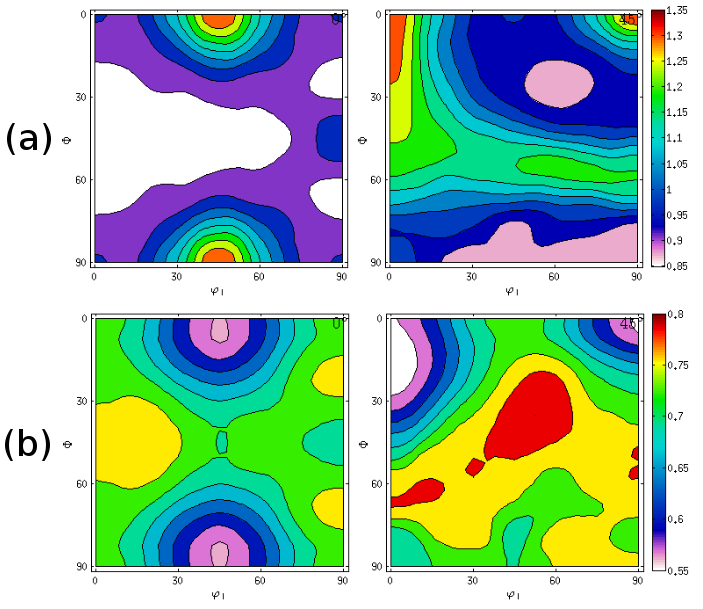
\includegraphics[width=0.9\textwidth]{IF75_ODF_Comp}
  \caption{(a) FDO del acero IF. (b) FDOG de ancho de pico del acero IF. En la sección $\phi_2 \ = \ 45$\,$^{\circ}$ puede apreciarse que las orientaciones de la fibra $\alpha$ exiben un ancho de pico menor, mientras que las orientaciones de la fibra $\gamma$ tienen un ancho claramente mayor. Adicionalmente parece que el mayor ensanchamiento se logra en orientaciones intermedias entre la fibra $\alpha$ y la $\gamma$ lo que es consistente con lo esperado para este material.}
  \label{fig:IFODFComp}
\end{figure}

Al comparar las secciones $\phi_2 \ = \ 45$\,$^{\circ}$ de la FDO y la FDOG puede apreciarse que a pesar de que la textura está definida por dos componentes principales, la fibra $\alpha$ y  la $\gamma$, los defectos no se acumularon equitativamente en ambas fibras, sino que los mismos fueron a parar a la fibra $\gamma$, mientras que la $\alpha$ acumuló una cantidad de defectos considerablemente menor.
El máximo en la FDOG se encuentra, sin embargo, en las orientaciones intermedias entre ambas fibras.

\newpage
\section{Estudio de la microestructura por EBSD}\label{S:IFEBSD}
Si se compara los resultados obtenidos en las secciones anteriores, puede verse que el método de Langford y el CMWP tienen una diferencia conceptual importante: mientras que el primero da la información microestructural relacionado con la orientación de los cristales, el segundo da esa información como función de la orientación de la muestra.
Si bien hay bases conceptuales para aceptar cualquiera de las dos suposiciones, las conclusiones que se obtienen de ambos modelos pueden llegar a ser contradictorias.
En ese sentido, las mediciones de EBSD, al permitir observar la microestructura más directamente, permitieron dar una base independiente para tratar de resoler cuál de los dos modelos representa más adecuadamente la microestructura del acero IF.

Las mediciones de EBSD se realizaron según lo especificado en la Sec. \ref{S:MatEBSD}, y permitieron obtener mapas como el que se observa en la Fig. \ref{fig:IFEBSD}.
En el mapa de figura de polo inversa pueden observarse que los granos (no confundir con el concepto de cristalita empleado en XRD) se encuentran alargados en la dirección de RD, como es de esperar para un material laminado.

\begin{figure}[!htb]
  \centering
  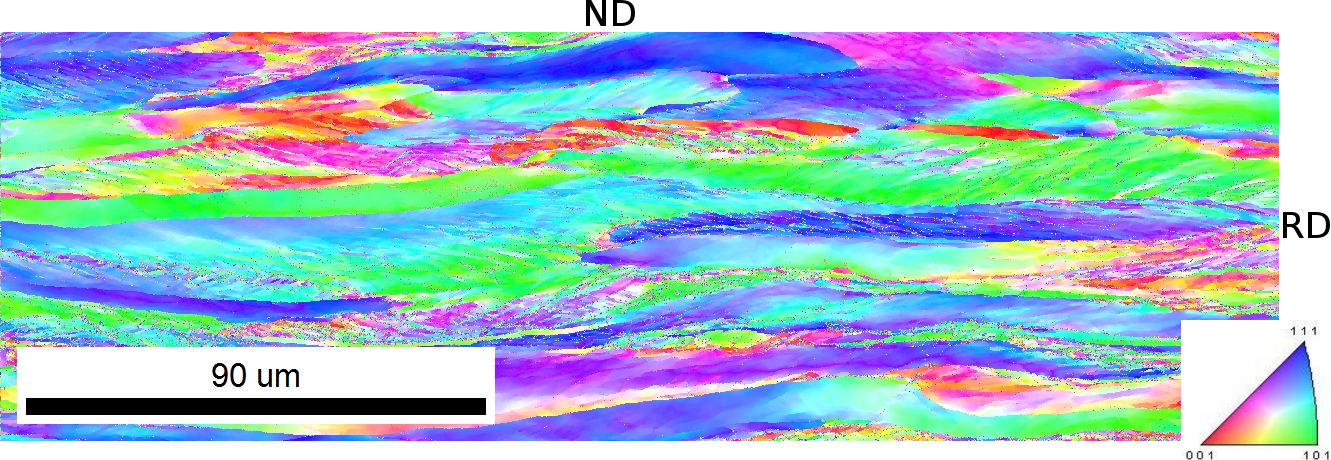
\includegraphics[width=\textwidth]{EBSD/IFEBSD}
  \caption{Mapa EBSD de figura de polo inversa EBSD del acero IF. La dirección de laminado RD es horizontal y la dirección normal a la chapa ND es hacia arriba. Puede verse como los granos tienen una forma ``alargada'' paralela con RD.}
  \label{fig:IFEBSD}
\end{figure}

Como se explicó en la Sec. \ref{S:MatEBSD}, a partir de un dado mapa de EBSD se puede calcular la FDO directamente, sin necesidad de realizar una inversión, como en el caso de XRD.
El problema que puede aparecer en las FDO obtenidas desde las mediciones de EBSD es que la estadística provista por un mapa suele ser insuficiente, y se puede cuestionar la representatividad de los datos microestructurales obtenidos a partir de cierto mapa.
En la Fig. \ref{fig:IFEBSDText} se muestran las FPs obtenidas a partir del mapa de EBSD que se muestra en la Fig. \ref{fig:IFEBSD}, que muestran un gran parecido cualitativo con las FPs obtenidas de las mediciones de XRD que se muestran en la Fig. \ref{fig:IFTextRawRec}.
El hecho de que las FP obtenidas de los mapas de EBSD sean más intensas y dispersas que las obtenidas por XRD se debe precisamente a la falta de estadística en las primeras, sin embargo el parecido entre ambas es suficiente como para asegurar que la comparación entre los resultados obtenidos de ambos experimentos es válida.

\begin{figure}[!htb]
  \centering
  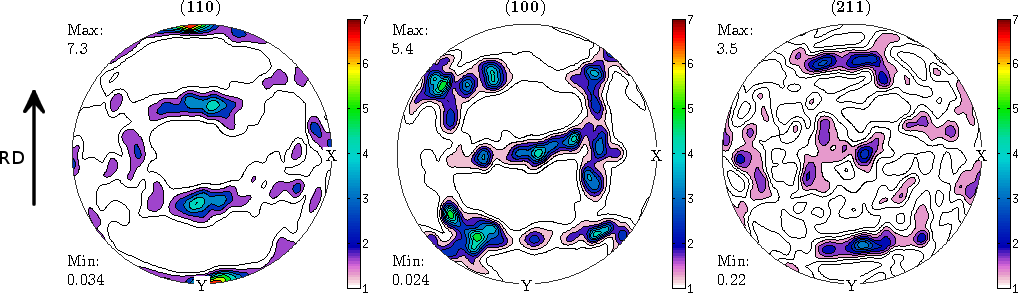
\includegraphics[width=\textwidth]{IF75_RDup}
  \caption{Figuras de polos calculadas a partir del mapa de EBSD mostrado en la Fig. \ref{fig:IFEBSD}. El parecido que guardan estas figuras de polos con las obtenidas a través de los experimentos de rayos X, que se muestran en la Fig. \ref{fig:IFFWHMRawRec}.}
  \label{fig:IFEBSDText}
\end{figure}

Para estudiar las características de la anisotropía de la microestructura del acero IF, se sacó provecho del hecho de que la mayoría de los cristales se encuentran en la fibra $\alpha$ o en la fibra $\gamma$.
Como primer paso se tomó cada mapa de EBSD y se crearon dos particiones, una con todos los cristales con su dirección [110] paralela a RD (fibra $\alpha$) y otra con el resto de los cristales.
Luego se realizaron dos particiones más, sólo que separando los cristales pertenecientes a la fibra $\gamma$, es decir, con su dirección [111] paralela a ND, y los que no pertenecían a dicha fibra, también partiendo del mapa original.
Una vez creados los cuatro mapas, que pueden verse en las imágenes de la Fig. \ref{fig:IFEBSDPar}, se procedió a determinar la microestructura de cada uno de ellos.
\begin{figure}[!htb]
  \centering
  \includegraphics[width=\textwidth]{EBSD/IFEBSD_Partitions}
  \caption{Para estudiar la anisotropía en la microestructura del acero IF se tomaron los mapas de EBSD y se comparó la microestructura de las orientaciones cuyos planos $\{110\}$ eran perpendiculares a RD (pertenecientes a la fibra $\alpha$ y las que no. Se hizo la misma comparación con las orientaciones del mismo mapa que tenían sus planos $\{111\}$ perpendiculares a ND (pertenecientes a la fibra $\gamma$) y las que no lo tenían.}
  \label{fig:IFEBSDPar}
\end{figure}

Para poder analizar la microestructura en un mapa de EBSD es fundamental realizar una reconstrucción de granos previo a cualquier estudio.
La reconstrucción de granos consiste en colocar un borde de grano entre dos píxeles que tienen una misorientación mayor a cierto ángulo, definido por el usuario, y que en este trabajo se consideró 5\,$^{\circ}$. Las propiedades de la microestructura que se decidieron estudiar fueron el tamaño de grano y la densidad de dislocaciones.

\nomenclature{GND}{Dislocaciones geométricamente necesarias}

El tamaño de grano se estimó a partir de la determinación de la longitud de intercepción media.
Dicho método consiste en trazar líneas y determinar la longitud promedio de los segmentos que surgen entre las intersecciones entre las líneas y los bordes de grano.
La densidad de dislocaciones se mide en función del modelo de \textit{Dislocaciones Geométricamente Necesarias (GND, por sus siglas en inglés)}\cite{Pantleon2008}, que estima la densidad de dislocaciones en el material de acuerdo a las misorientaciones de los cristales vecinos.
Si bien ninguno de estos dos conceptos es estrictamente igual a los que se miden cuando realiza LPA, es una suposición razonable que el comportamiento cualitativo debería respetarse, es decir, si los granos que pertenecen a la fibra $\gamma$ tienen menor cantidad de dislocaciones, medidas a través de LPA, deberían tener menor cantidad de GNDs, medidas a partir de un mapa de EBSD.

En la Fig. \ref{fig:IFEBSDVs} se muestran gráficas de las cuatro particiones mencionadas, comparando el tamaño de grano (a) y densidad de dislocaciones (b).

\begin{figure}[!htb]
  \centering
  \includegraphics[width=\textwidth]{EBSD/IFEBSD_Size_GND}
  \caption{(a) Comparación del tamaño promedio de granos, medido según el método de longitud de intercepciones para las particiones de la Fig. \ref{fig:IFEBSDPar}. (b) Comparación de las dislocaciones geométricamente necesarias (GND) acumuladas en las particiones creadas.}
  \label{fig:IFEBSDVs}
\end{figure}

Observando la Fig. \ref{fig:IFEBSDVs}-a puede verse que los granos que pertenecen a la fibra $\alpha$ son más grandes que los que pertenecen a la fibra $\gamma$, más allá de la dispersión calculada a partir del mapa, y por un factor de aproximadamente 2.5.
Dado que un mayor tamaño de grano se vincula con un menor ensanchamiento de pico, este resultado es consistente con el observado en la FDOG de FWHM mostrada en la Fig. \ref{fig:IFODFComp}.
Adicionalmente, el tamaño de grano que se obtiene para los granos que no pertenecen a la fibra $\alpha$, se acerca al que resulta a partir de considerar los granos que no pertenecen a la fibra $\gamma$, como es razonable esperar.

A partir de la analizar los dos histogramas que aparecen en la Fig. \ref{fig:IFEBSDVs}-b se obtienen conclusiones parecidas, ya que el valor promedio de la distribución de GND para las orientaciones pertenecientes a la fibra $\alpha$ de 1.30 10$^{14}$\,m$^{-2}$, es claramente menor al obtenido tomando sólo las orientaciones pertenecientes a la fibra $\gamma$, que es igual a 1.79 10$^{14}$\,m$^{-2}$.
Es más, la propia distribución de GND de las orientaciones pertenecientes a la fibra $\gamma$ es más ancha, con muchos más valores altos que la distribución de las orientaciones que pertenecen a fibra $\alpha$, explicando por qué el promedio de una es mayor que el de la otra, más allá de que la moda de ambas distribuciones es parecida.
Finalmente, puede verse que las distribuciones complementarias son parecidas, es decir que la distribución de GND de las orientaciones que no pertenecen a la fibra $\alpha$ es parecida a la distribución de orientaciones que pertenecen a fibra $\gamma$, y viceversa.
\section{Discusión de resultados}\label{S:IFDis}
Como se dijo al principio de la Sec. \ref{S:IFCMWP}, el método de Langford y el CMWP no sólo difieren en la forma en que presentan los datos, sino que ambos modelan de forma conceptualmente distinta la anisotropía en la microestructura de los materiales.
Mientra el primer método considera que la anisotropía está vinculada fundamentalmente con la orientación de los cristales caracterizada por la textura, el segundo considera que las cristalitas tienen forma esférica y que la anisotropía en los ensanchamientos no tiene relación con la textura, sino que es consecuencia de variaciones en el factor de contraste, es decir, la anisotropía de ensanchamiento es una consecuencia geométrica, definida por la relación entre el vector de Burgers de una dislocación y el vector de difracción.
Como consecuencia de esto, la acumulación de defectos no depende de la textura, sino de la orientación de la muestra.
De alguna manera, esta conclusión es inevitable si se tiene en cuenta que expresiones como la Ec. \ref{eq:Cav2}, que son las empleadas en el software CMWP, se obtienen a partir de la suposición de que el material no tiene textura y de que todos los sistemas de deslizamiento están igualmente poblados.

Desde luego la suposición de que el material no tiene textura claramente no se puede aplicar a este material, sin embargo puede considerarse que todos los sistemas de deslizamiento están igualmente poblados en materiales cúbicos, ya que éstos poseen pocos sistemas de deslizamiento activos.
El problema que tiene este modelo para estudiar la densidad de dislocaciones del material, es que debido a las suposiciones en que se basa, predice que la densidad de dislocaciones debe ser uniforme para todo el material, lo que no parece corresponder con la FPG que se observa en la Fig. \ref{fig:IFCMWPrho}-b, a menos que se considere que la precisión del método CMWP para estimar densidad de dislocaciones sólo permite estimar el orden de magnitud de dicha cantidad.
Notar que este es un problema parecido al que se le presentó a Kamminga et al en \cite{mittemeijer2003diffraction}, y que fue abordado en la Sec. \ref{SS:Langford}.

Por otro lado, suponer que el tamaño de cristalita depende solamente de la orientación de la muestra resulta verosímil al ver los mapa de EBSD, donde se ve que la forma de los granos está claramente condicionada por la forma en que el material fue deformado, aunque siempre debe recordarse que el concepto de grano definido por la metalografía o EBSD es diferente al concepto de cristalita derivado de los experimentos de XRD, ya que ambos surgen de interacciones físicas completamente diferentes.

Sin embargo, es claro que el factor de contraste contribuye al menos parcialmente al efecto de ensanchamiento anisotrópico, aunque no queda claro en qué medida, y el no tomar en cuenta este factor es una de las críticas que se le puede hacer al método de Langford.

La otra crítica que se puede hacer es que la en la reconstrucción de la FDOG de FWHM se tienen que emplear datos con elevado error, ya que el ancho de pico es una cantidad difícil de estimar apropiadamente cuando el pico tiene poca intensidad.
Si bien esto también ocurre en alguna medida cuando se miden FPs, en el caso de la textura los datos menos confiables son los valores más pequeños de la FP, por lo que su contribución a la FDO es menor.
En el caso de la FPG de FWHM ocurre que los los picos de menor intensidad tienden a ser de los que poseen mayor FWHM, por  lo que en la FPG, lo valores más elevados pueden ser los menos confiables, lo que a su vez reduciría la confiabilidad de la FDOG obtenida a partir de las FPG.

\begin{figure}[!htb]
  \centering
  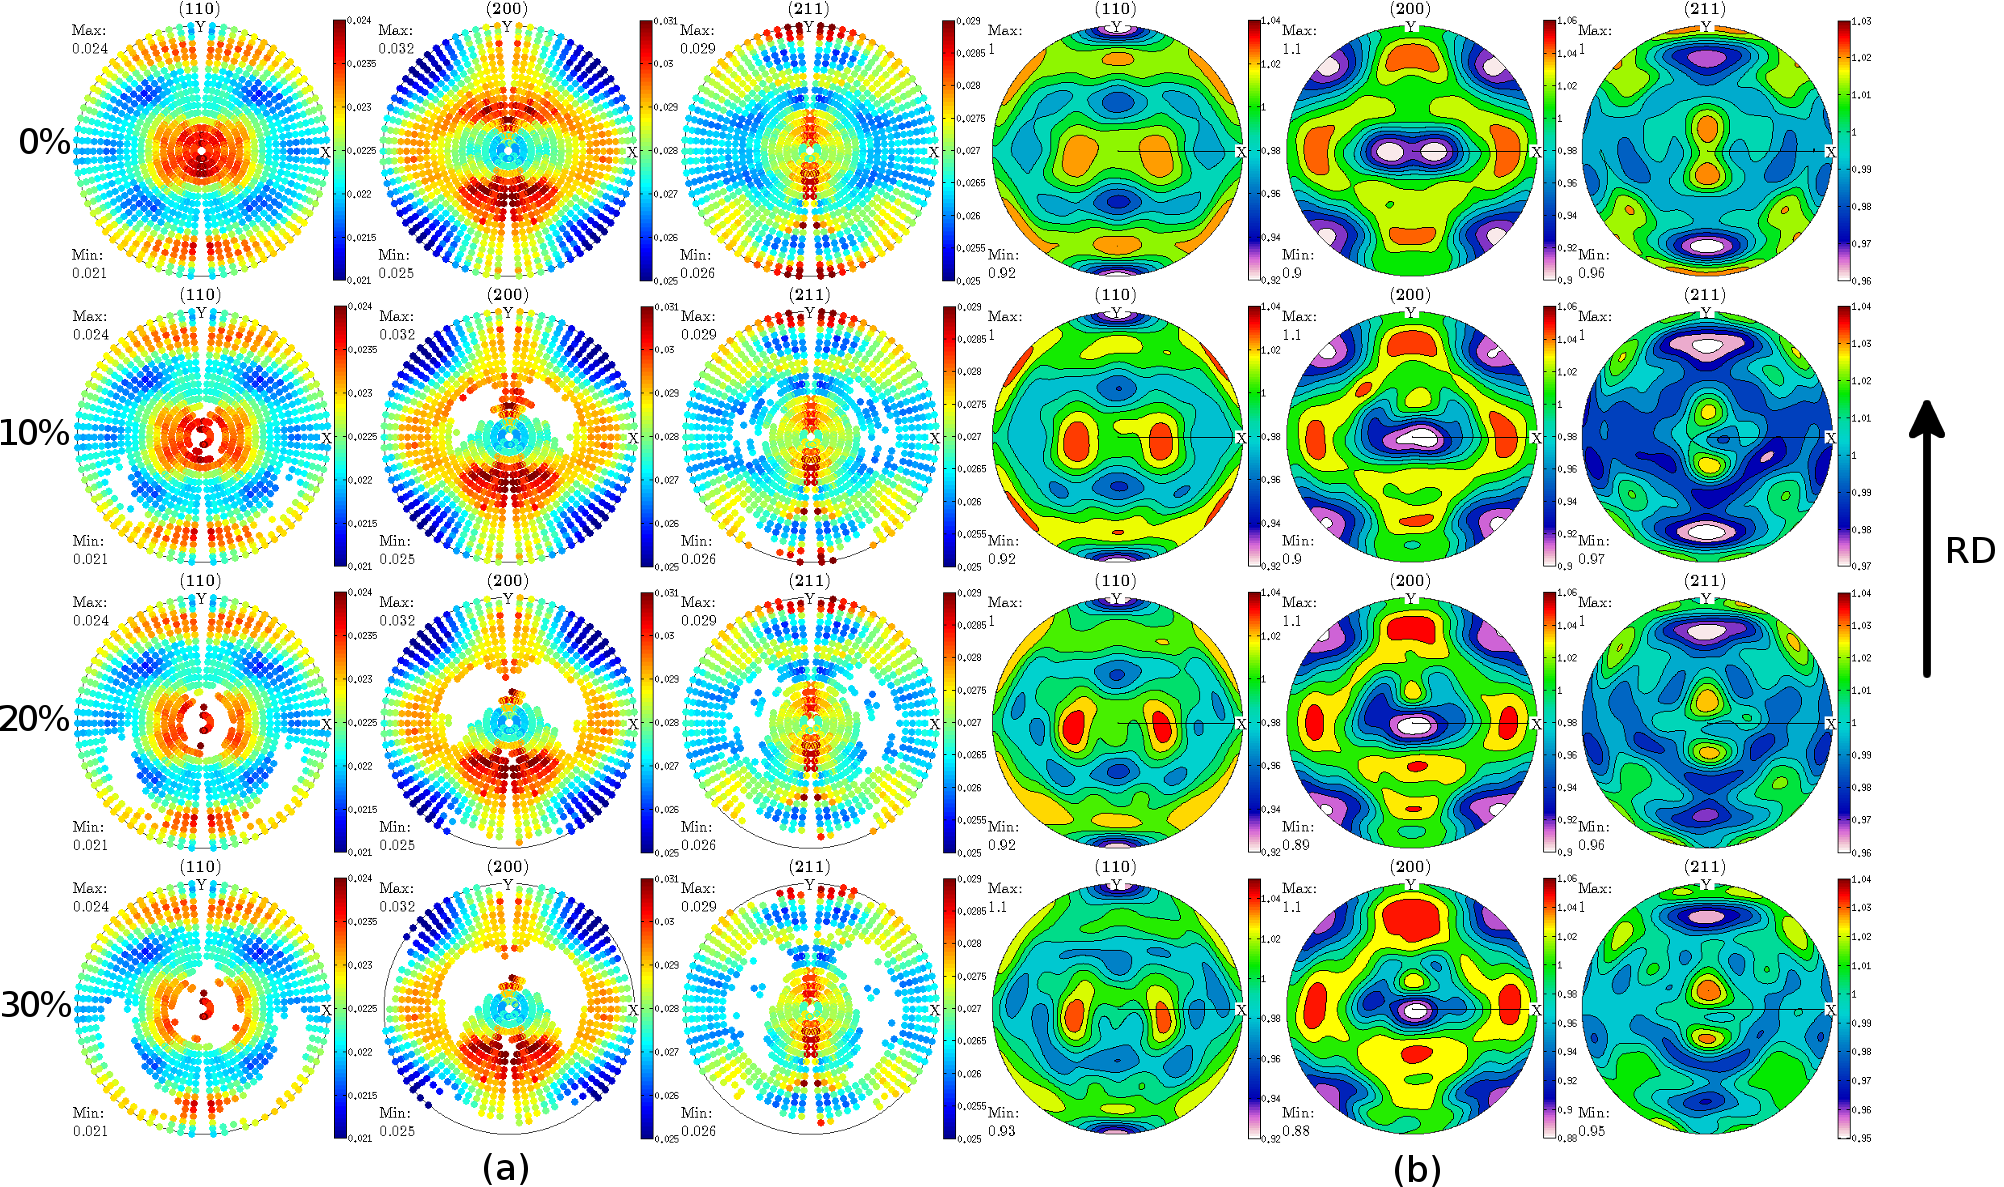
\includegraphics[width=\textwidth]{Quitandodatos}
  \caption{Figuras de polos recalculadas para distintos datos de entrada. Para verificar la consistencia de las FDOs calculadas se fueron removiendo datos en las FPGs de FWHM, con base a la intensidad de la FP de intensidad. Los porcentajes que figuran en la imagen indican que se removieron los FWHM que correspondían a puntos que están en el 0\,\%, 10\,\%, 20\,\%, 30\,\% de la distribución de intensidad en las FPs, ya que esos FWHM son lo que tienen mayor error.}
  \label{fig:IFFWHMRecvsCrop}
\end{figure}

Para poner a prueba la importancia que tienen estos valores poco confiables en la construcción de la FDOG, se decidió analizar cómo varía la reconstrucción de las FPGs de FWHM cuando se remueven de la FPG experimental los valores de FWHM que provienen de los picos de menor intensidad.
El proceso se repitió removiendo el 10\,\%, 20\,\%, y 30\,\% de los valores menos intensos, y como se puede ver en la progresión de la Fig. \ref{fig:IFFWHMRecvsCrop}, si bien se puede observar pequeñas variaciones en las FPGs recalculadas, la relaciones cualitativas se mantienen intactas, aún cuando se remueve tanto como el 30\,\% de los datos, lo que resulta en un apoyo importante al método de Langford.

Finalmente, cuando se tienen en cuenta los resultados obtenidos por EBSD, puede verse que cuando se analiza la microestructura a partir de la misorientación de los cristales, la conclusión es que los granos que pertenecen a la fibra $\alpha$ son en promedio más grandes y con menor cantidad de dislocaciones que los que pertenecen a la fibra $\gamma$, lo que implica que los experimentos de EBSD predicen que los picos que se obtendrían de realizar experimentos de XRD sobre los granos que pertenecen a la fibra $\alpha$ deberían ser más angostos que los que se medirían si se hiciera un experimento de difracción sólo con los cristales que pertenecen a la fibra $\gamma$, en acuerdo con lo que se observó en la FDOG de FWHM en la Fig. \ref{fig:IFODFComp}, en apoyo al método de Langford.
El acuerdo entre el método de Langford y las mediciones de EBSD resulta más importante si se recuerda que los datos de microestructura obtenidos por EBSD son completamente independientes de los obtenidos por XRD, y que, a pesar de que la estadística provista por los experimentos de EBSD es menor que la de XRD, las FDO que se obtienen con ambas técnicas son lo suficientemente similares como para sostener que ambas dan información igualmente representativa de lo que ocurre con la microestructura de la muestra.

Habiendo observado la buena correlación que existe entre las variaciones de ancho de pico y la textura del material, se decidió dar un paso más con el método de Langford, que consistió en emplear las Ecs. \ref{eq:Gauss}, \ref{eq:Lorentz} y \ref{eq:Hg} para generar FPG de tamaño y deformación a partir de las mediciones de FWHM y factor de mezcla $\eta$.
Las FPG de tamaño y deformación fueron empleadas para generar las FDOG de tamaño y deformación que se muestran en la Fig. \ref{fig:IFMicroRecocido}, y este análisis se hizo tanto para la muestra laminada como para tres muestras que fueron recocidas a diferentes temperaturas después del laminado.
Todas las muestras fueron recocidas por 5 minutos, y las temperaturas de recocido fueron 400\,$^{\circ}$C, 600\,$^{\circ}$C y 750\,$^{\circ}$C, respectivamente.

\begin{figure}[!htb]
  \centering
  \includegraphics[width=\textwidth]{IF75_ODF_Comp_Rec}
  \caption{Ancho de pico vs recocido}
  \label{fig:IFMicroRecocido}
\end{figure}

Puede verse que los recocidos a 400\,$^{\circ}$C y 600\,$^{\circ}$C no tienen mayor efecto sobre la textura, mientras que el recocido a 700\,$^{\circ}$C elimina casi por completo la componente Goss de la textura, y reduce notablemente la fibra $\alpha$, es decir que después del recocido a 750\,$^{\circ}$C la componente $\gamma$ es la única que queda, tal como se suele esperar en este acero.

La observación de las FDOG de tamaño y deformación de la muestra laminada dan resultados coherentes con lo que se observó en la FDOG de FWHM en la Fig. \ref{fig:IFODFComp}, ya que puede verse como la fibra $\gamma$ acumula más deformación que la $\alpha$, y que esta última tiene dominios más grandes que la primera.
Notablemente, también puede verse como la deformación acumulada se mantiene siempre en la fibra $\gamma$, aunque reduciendo su valor con la temperatura de recocido.
También puede verse que la temperatura de recocido tiene el efecto de homogeneizar la distribución de los tamaños de dominio, aunque no se ven mayores cambios entre las FDOG de tamaño de los recocidos a 400\,$^{\circ}$C y 600\,$^{\circ}$C.
Esto implica que las menores temperaturas de recocido aportan suficiente energía como para aniquilar las dislocaciones en las orientaciones más cargadas, que son las que se encuentran a lo largo de la fibra $\gamma$, pero dicha energía no es suficiente como para reorientar los cristales ni para hacerlos crecer, razón por la cual la textura y la FDOG de tamaño no se modificaron en gran medida.

En el recocido a 750\,$^{\circ}$C puede verse un comportamiento completamente distinto, ya que se observa como las orientaciones que no pertenecen a la fibra $\gamma$ desaparecieron casi completamente, y que las FDOG de tamaño y deformación se homogeneizaron casi completamente.
Esto significa que a 750\,$^{\circ}$C, no sólo se aniquilan las dislocaciones, sino que los dominios orientados según la fibra $\gamma$ crecen a expensas de los dominios más grandes que tienen orientaciones menos favorables.

Si se analizan las muestras recocidas por medio de la técnica de EBSD, la tendencia observada es la misma que la observada a través del método de Langford.
Sin embargo, dada la anisotropía introducida por el laminado, es de esperar que los tamaños de dominio EBSD muestren también una anisotropía de muestra.
En la Fig. \ref{fig:VlyHl} puede verse la variación de los tamaños de dominio para la muestra deformada en frío y para las tres temperaturas de recocido, separadas por componente de textura.
En la Fig. \ref{fig:VlyHl}-a se muestra la longitud horizontal (a lo largo de RD) promedio de los granos, mientras que en la Fig. \ref{fig:VlyHl}-b se hace lo mismo para la longitud vertical (a lo largo de ND).

\begin{figure}[!htb]
  \centering
  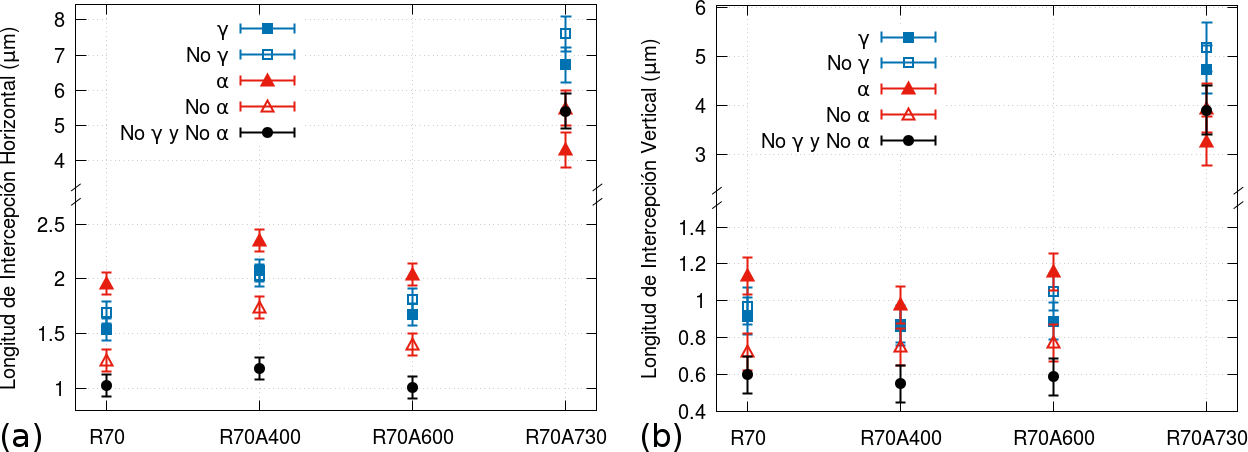
\includegraphics[width=\textwidth]{EBSD/VlenyHlen}
  \caption{Tamaño de grano horizontal y vertical.}
  \label{fig:VlyHl}
\end{figure}

En ambas figuras puede verse como los granos que están orientados según la fibra $\alpha$ son siempre más grandes que los orientados según la fibra $\gamma$.
Esto es cierto para todas las temperaturas de recocido menores a 730\,$^{\circ}$, mientras que para esta temperatura de recocido la situación se invierte.
Recordando la Ec. \ref{eq:Lorentz} puede verse que a mayor tamaño de grano, el método de Langford predice un ensanchamiento de pico menor, es decir, que los cristales orientados según la fibra $\alpha$ deberían exhibir un ensanchamiento de pico que los de la fibra $\gamma$, que es precisamente lo que se observa en este caso.
Si se observa la FDOG de tamaño para la muestra recocida a 730\,$^{\circ}$ en la Fig. \ref{fig:IFMicroRecocido}, puede verse que para esa muestra, la FDOG no exhibe ninguna estructura apreciable, lo que implica que o bien el tamaño de cristalita no se encuentra correlacionado con la textura del material, o que el tamaño de cristalita ha crecido a un punto tal que hace que el ancho de pico sea demasiado pequeño como para ser resuelto por la metodología de Langford.

De la misma manera que se repitieron los análisis de tamaño de grano a partir del estudio la longitud de intercepción promedio, el análisis de la evolución de las GND con la temperatura de recocido también demostró resultados coherentes con los observados en la Fig. \ref{fig:IFMicroRecocido}.
En la Fig. \ref{fig:GNDyVH}-a puede verse que las orientaciones pertenecientes a la fibra $\gamma$ siempre poseen, en promedio, más dislocaciones que las orientaciones de la fibra $\alpha$, y que la densidad de GND se mantiene aproximadamente constante para temperaturas de recocido menores a 730\,$^{\circ}$.
Cuando las muestras son recocidas a 730\,$^{\circ}$ se observa un descenso marcado en la densidad de dislocaciones, así como una pérdida de correlación entre la densidad de dislocaciones y las componentes de textura analizadas.

\begin{figure}[!htb]
  \centering
  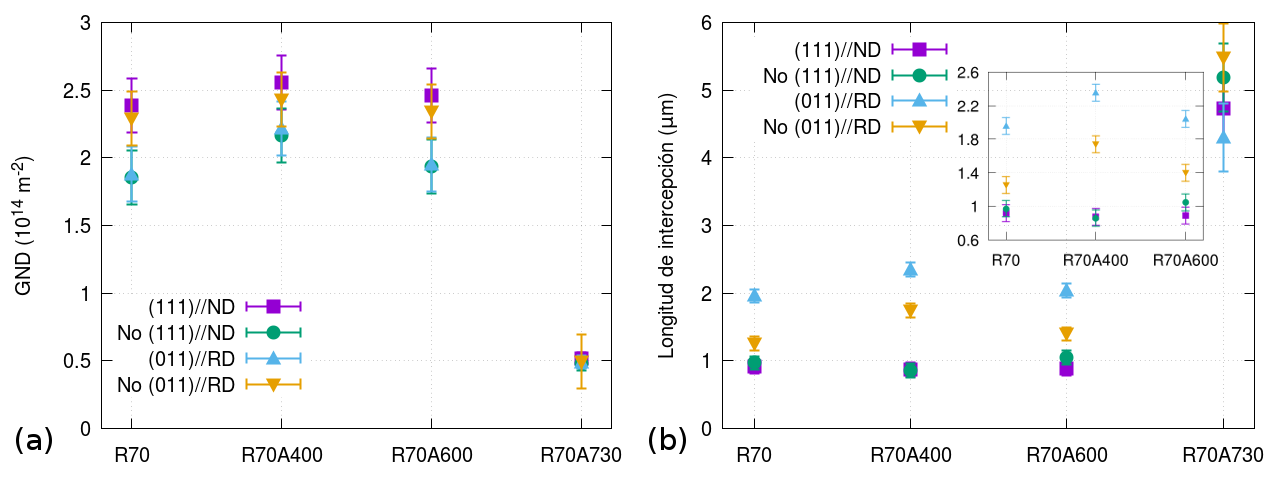
\includegraphics[width=\textwidth]{EBSD/GNDyVHvsT}
  \caption{GND y Tamaño de grano.}
  \label{fig:GNDyVH}
\end{figure}

Por último, cabe mencionar que para comparar mejor los resultados de tamaño obtenidos en EBSD con los de XRD, es más correcto comparar las longitudes medidas a lo largo de RD cuando se analiza la fibra $\alpha$, con las medidas a lo largo de ND para las orientaciones pertenecientes a la fibra $\gamma$, como se hace en la Fig. \ref{fig:GNDyVH}-b.
Como era previsible al observar las mediciones de la Fig. \ref{fig:VlyHl}, las diferencias observadas entre las fibras $\alpha$ y $\gamma$ se vuelven más notables, tanto para la muestra laminada en frío como para las muestras recocidas a temperaturas menores a 730\,$^{\circ}$, mientras que para la muestra recocida a 730\,$^{\circ}$ la correlación entre tamaño de grano y componente de textura se pierde completamente, en consonancia con lo observado en las FDOG de la Fig. \ref{fig:IFMicroRecocido}.




\section{Conclusiones}\label{S:IFConclusiones}
Se deformó un acero libre de intersticiales por laminado hasta lograr una reducción de la sección transversal del 75\,\%, y se estudió su microestructura por medio de mediciones de EBSD y de difracción de rayos X.
Los datos obtenidos por difracción de rayos X fueron analizados siguiendo el modelo de Langford y el de CMWP.
Mientras el primer método atribuye el ensanchamiento anisotrópico a diferencias en la acumulación de defectos dadas por la textura, el segundo considera que dicha anisotropía se debe únicamente a razones geométricas, por lo que considera que la microestructura depende únicamente de la orientación de la muestra y no de la textura de la misma.

La textura de este acero era la esperada para un material BCC deformado, con las orientaciones acumuladas principalmente en dos componentes, las llamadas fibra $\alpha$ y fibra $\gamma$.

El método de Langford de figuras de polos generalizadas indicó que los defectos tienden a acumularse en la fibra $\gamma$, ya que es en esta región del espacio de orientaciones en que la FDOG de FWHM tiene sus valores máximos, mientras que las orientaciones correspondientes a la fibra $\alpha$ este función tiende a anularse, lo que debe interpretarse como que la fibra $\alpha$ posee cristalitas de mayor tamaño y con menos dislocaciones.

El método CMWP también indica que los dominios más grandes son lo que han acumulado más dislocaciones, pero en vez de atribuir dichos dominios a una componente de textura, los coloca en la orientaciones de la muestra que son paralelas a la dirección (110).

Se realizaron mediciones de EBSD para tener una caracterización independiente de la microestructura que permitiera dilucidar cuál de los dos modelos representa mejor la microestructura del material, encontrándose un mejor acuerdo con el modelo de Langford que con el CMWP, lo que parecería indicar que aunque el primer método no toma en cuenta la contribución de los factores de contraste al ensanchamiento de los picos, resulta más adecuado para describir la anisotropía de la microestructura en materiales con textura que el método CMWP, que emplea un modelo cuantitativo para calcular los factores de contraste a costa de despreciar las contribuciones de la textura al ensanchamiento de los picos.
